\documentclass[a4paper,parskip,11pt, DIV12]{scrreprt}

\usepackage[english]{babel} % Für Deutsch [english] zu [ngerman] ändern. 
\usepackage[utf8]{inputenc}
\usepackage[T1]{fontenc}
\usepackage{blindtext}
\usepackage{graphicx}
\usepackage{subfigure}
\renewcommand{\familydefault}{\sfdefault}
\usepackage{helvet}
\usepackage{fancyhdr}
\usepackage{amsmath}
\usepackage{mdwlist} %Benötigt für Abstände in Aufzählungen zu löschen
\usepackage{here}
\usepackage{calc}
\usepackage{hhline}
\usepackage{marginnote}
\usepackage{chngcntr}
\usepackage{tabularx}
\usepackage{titlesec} % Textüberschriften anpassen

% \titleformat{Überschriftenklasse}[Absatzformatierung]{Textformatierung} {Nummerierung}{Abstand zwischen Nummerierung und Überschriftentext}{Code vor der Überschrift}[Code nach der Überschrift]

% \titlespacing{Überschriftenklasse}{Linker Einzug}{Platz oberhalb}{Platz unterhalb}[rechter Einzug]

\titleformat{\chapter}{\LARGE\bfseries}{\thechapter\quad}{0pt}{}
\titleformat{\section}{\Large\bfseries}{\thesection\quad}{0pt}{}
\titleformat{\subsection}{\large\bfseries}{\thesubsection\quad}{0pt}{}
\titleformat{\subsubsection}{\normalsize\bfseries}{\thesubsubsection\quad}{0pt}{}

\titlespacing{\chapter}{0pt}{-2em}{6pt}
\titlespacing{\section}{0pt}{6pt}{-0.2em}
\titlespacing{\subsection}{0pt}{5pt}{-0.4em}
\titlespacing{\subsubsection}{0pt}{-0.3em}{-1em}

%\usepackage[singlespacing]{setspace}
%\usepackage[onehalfspacing]{setspace}

\usepackage[
%includemp,				%marginalien in Textkörper einbeziehen
%includeall,
%showframe,				%zeigt rahmen zum debuggen		
marginparwidth=25mm, 	%breite der marginalien
marginparsep=5mm,		%abstand marginalien - text
reversemarginpar,		%marginalien links statt rechts
%left=50mm,				%abstand von Seitenraendern
%			top=25mm,				%
%			bottom=50mm,
]{geometry}		

%Bibliographie- Einstellungen
\usepackage[babel,german=quotes]{csquotes}
\usepackage[
backend=bibtex8, 
natbib=true,
style=numeric,
sorting=none
]{biblatex}
\bibliography{Quelle}
%Fertig Bibliographie- Einstellungen

\usepackage{hyperref}

\newenvironment{conditions}
{\par\vspace{\abovedisplayskip}\noindent\begin{tabular}{>{$}l<{$} @{${}={}$} l}}
	{\end{tabular}\par\vspace{\belowdisplayskip}}
	
\begin{document}
	
	\begin{titlepage}
		\begin{figure}[H]
			\hfill
			\subfigure{
\includegraphics[scale=0.04]{uzh}}
		\end{figure}
		\vspace{1 cm}
		\textbf{\begin{huge}KT I Lab Course
		\end{huge}}\\
		\noindent\rule{\textwidth}{1.1 pt} \\
		
		\begin{Large}\textbf{Angular Correlation}
		\end{Large}\\ 
		\normalsize 
		\par
		\begingroup
		\leftskip 0 cm
		\rightskip\leftskip
		\textbf{Assistant:}\\ Alexander Kish \\ \\
		\textbf{Students:}\\ Fabian Stäger, Manuel Sommerhalder \\ \\
		\textbf{Date of experiment:}\\ 24.01.2018 \\ \\
		\par
		\endgroup
		\clearpage
		
		
		
	\end{titlepage}
	
%Start Layout
	\pagestyle{fancy}
	\fancyhead{} 
	\fancyhead[R]{\small \leftmark}
	\fancyhead[C]{\textbf{Angular Correlation} } 
	\fancyhead[L]{
\includegraphics[height=2\baselineskip]{uzh}}
	
	\fancyfoot{}
	\fancyfoot[R]{\small \thepage}
	\fancyfoot[L]{}
	\fancyfoot[C]{}
	\renewcommand{\footrulewidth}{0.4pt} 
	
	\addtolength{\headheight}{2\baselineskip}
	\addtolength{\headheight}{0.6pt}
	
	
	\renewcommand{\headrulewidth}{0.6pt}
	\renewcommand{\footrulewidth}{0.4pt}
	\fancypagestyle{plain}{				% plain redefinieren, damit wirklich alle seiten im gleichen stil sind (ausser titlepage)
		\pagestyle{fancy}}
	
	\renewcommand{\chaptermark}[1]{ \markboth{#1}{} } %Das aktuelle Kapitel soll nicht Gross geschriben und Nummeriertwerden
	
	\counterwithout{figure}{chapter}
	\counterwithout{table}{chapter}
	%Ende Layout
	

\chapter{Experimental Results}
For each angle in the range of $60^{\circ}$ to $180^{\circ}$ with steps of $15^{\circ}$ we took three 20 minute measurements: The number of coincident events measured with the software Maestro $r_m$, the number of coincident events measured by one of the scalers $r_s$, and the total number of events measured by the fixed detectors $r_{tot}$. The results of these measurements for each angle are listed in table \ref{tab:measurement}. 
%
\begin{table}[H]
\begin{center}
\begin{tabular}{lllll}
Angle $\theta$ [$^{\circ}$] & $r_{m}$ [Hz] & $r_{s}$ [Hz] & $r_{tot}$ [Hz]\\
\hline
60 	& 3.54 & 4.34 & 1470\\
75 	& 3.35 & 4.09 & 1469\\
90 	& 3.33 & 4.12 & 1469\\
105 	& 3.39 & 4.16 & 1468\\
120	& 3.44 & 4.20 & 1464\\
135	& 3.52 & 4.29 & 1464\\
150	& 3.60 & 4.35 & 1468\\
165	& 3.57 & 4.35 & 1466\\
180	& 3.67 & 4.31 & 1453\\ 
\end{tabular}
\label{tab:measurement}
\end{center}
\end{table}
%
The software Maestro gave us not only the number of coincident events as listed in the table above, but the number of events for a 8191 ADC channels. As an example, the histogram for $\theta = 90^{\circ}$ is shown in figure \ref{fig:histogramraw}, the rest can be found in the appendix.
%
\begin{figure}[H]
\centering
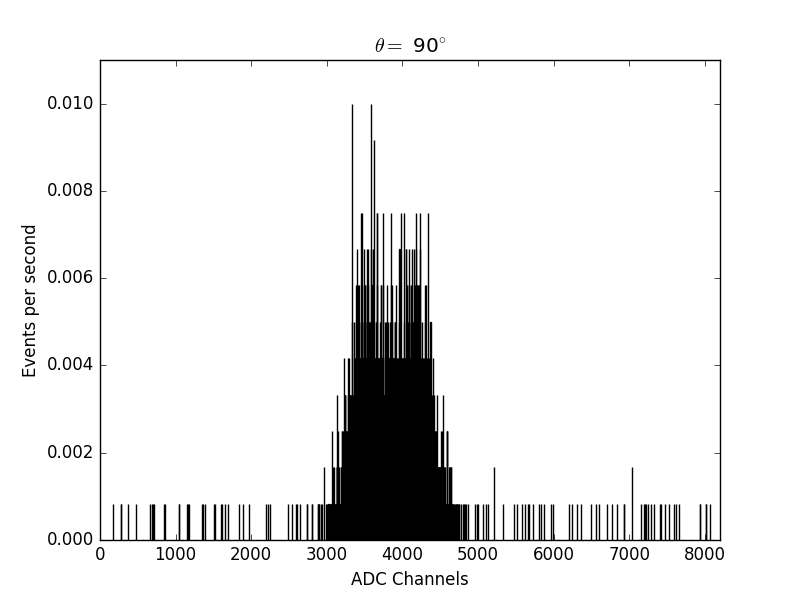
\includegraphics[scale=0.4]{plots/90degraw.png}
\caption[Histogram]{Histogram with ADC channels for $\theta = 90^{\circ}$}
\label{fig:hist120}
\end{figure}
%



\chapter{Data Analysis}
Since each measurement lasted for 20 minutes, the statistical errors on these measurements should be negligible. To check this assumption we calculated the statistical uncertainty on the measurement made by scaler 1 (BIG NUMBERS). Since scaler 1 was counting the number of events registered by the fixed detector, we would expect it to measure the same value in each of the $n$ measuring periods. The relative statistical uncertainty can thus be calculated by
%
\begin{align}
\frac{u_r}{\overline{r}} = \frac{1}{\overline{r}}\sqrt{\frac{\sum_i (r_i - \overline{r})^2}{n(n-1)}} \approx 0.1\%
\end{align}
%
Assuming the same statistical uncertainty on the Maestro data $r_m$ which consists of values in a range of $5\%$ around their mean, this statistical uncertainty can indeed be neglected.



We started by rescaling the x-axis from ADC channels to time. To make sure there are enough counts per bin we had to rebin the data. We merged 20 bins to one, giving us a time resolution of $0.22\,$ns. We then used the $\chi^2$-method to fit a Gaussian function on each histogram, taking into account an uncertainty on each bin of 
%
\begin{align}
u_{bin} = \sqrt{n_{bin}}
\end{align}

Figure \ref{fig:hist120} shows the histogram with Gaussian fit for the angle $\theta = 90^{\circ}$.
%
\begin{figure}[H]
\centering
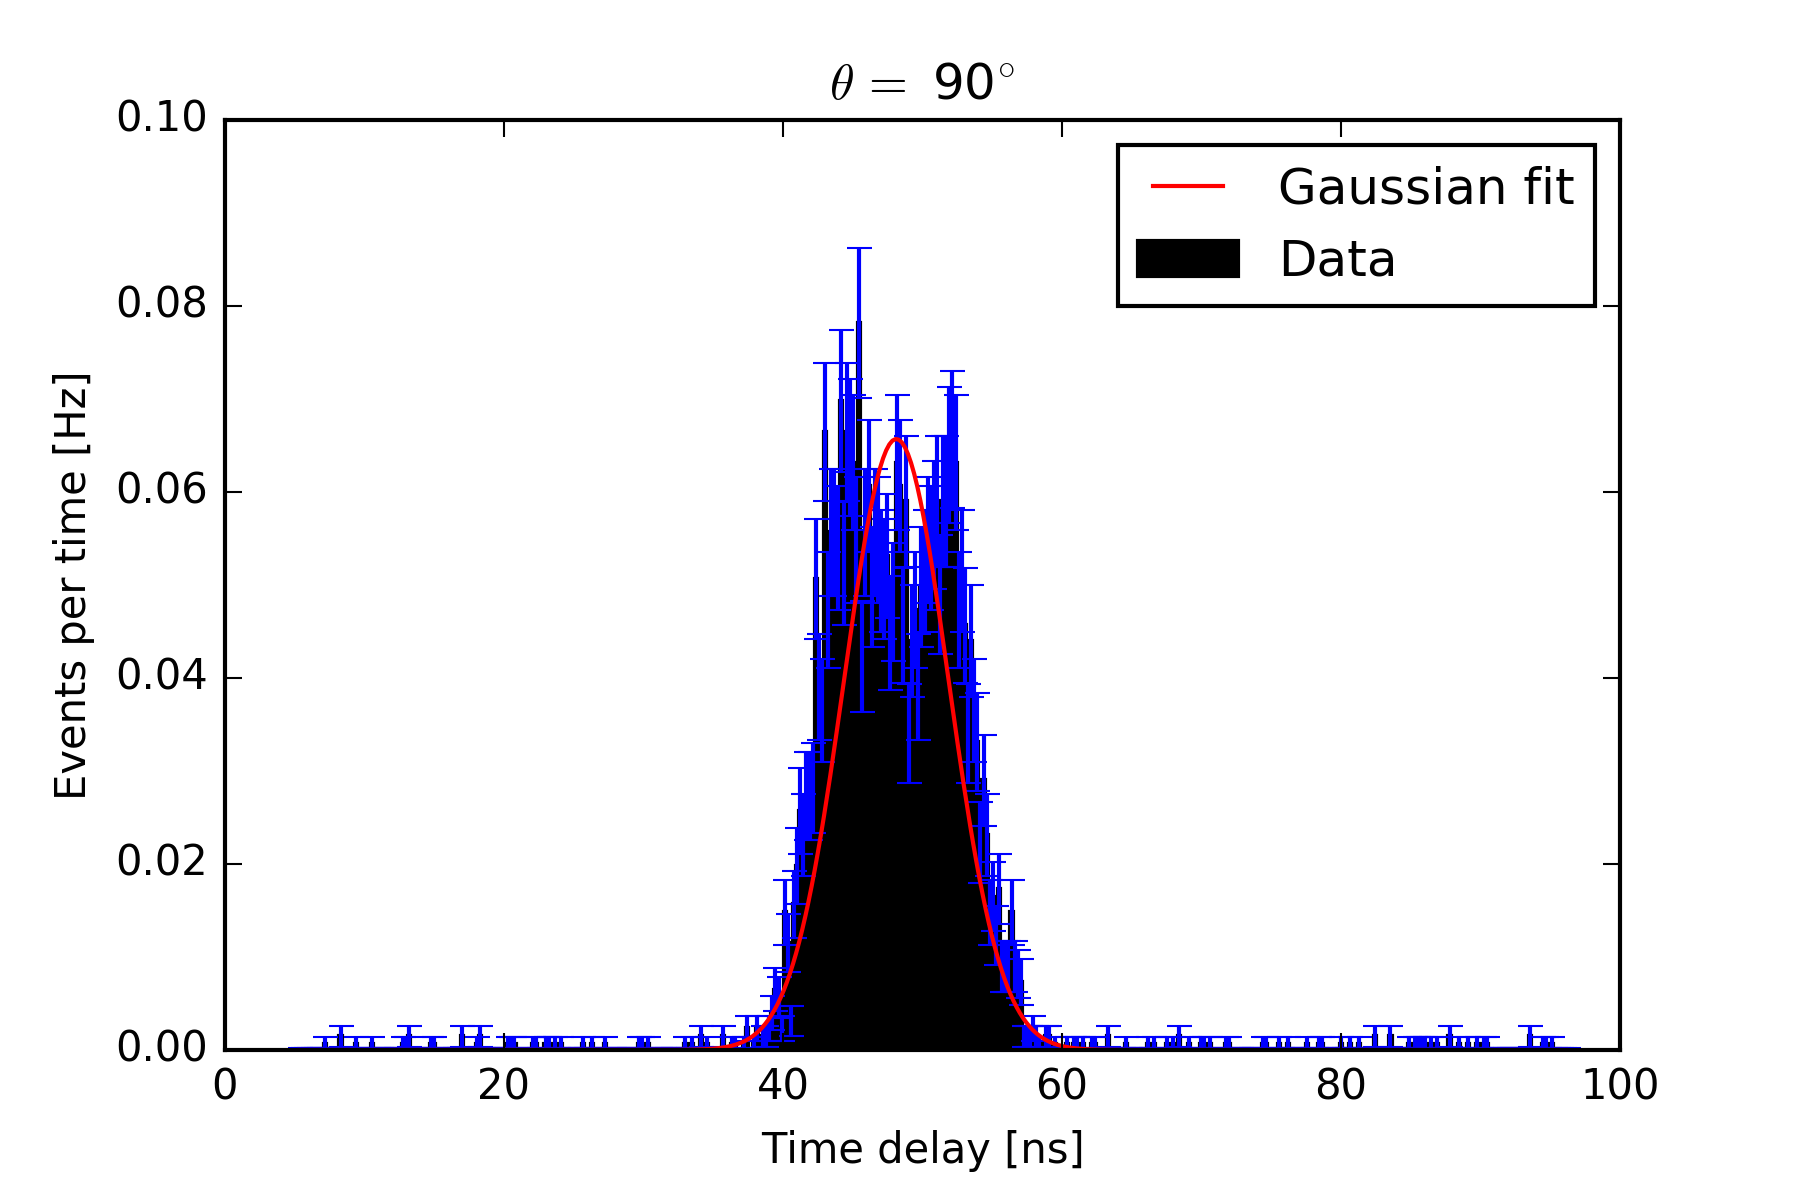
\includegraphics[scale=0.65]{plots/90deg.png}
\caption[Histogram]{Histogram with Gaussian Fit for angle $\theta = 90^{\circ}$}
\label{fig:hist120}
\end{figure}
%
We noticed that the measured data does not show a single peak at the set delay time, but instead two peaks slightly below and above. WHY? In a next step, we subtracted the background from the data. In order to estimate the background, we took the average of the bins in a range of [$3\sigma$, $4\sigma$] on both sides of the mean $\mu$. Then we subtracted this average from each bin in the histogram. We then summed all the bins in the histogram to get the number of coincident events per second $r_c$ for each angle. Table \ref{tab:nevents} shows the result for each angle compared to the number of coincident events per second $r_{s}$ as measured by the scaler.
%
\begin{table}[H]
\begin{center}
\begin{tabular}{llll}
Angle $\theta$ [$^{\circ}$] & $r_{c}$ [Hz] & $r_{s}$ [Hz]\\
\hline
60 	& 3.39 & 4.34\\
  75 	& 3.22 & 4.09\\
  90 	& 3.25 & 4.12\\
105 	& 3.33 & 4.16\\
120	& 3.37 & 4.20\\
135	& 3.44 & 4.29\\
150	& 3.48 & 4.35\\
165	& 3.49 & 4.35\\
180	& 3.54 & 4.31\\ 
\end{tabular}
\caption{Rate for each angle}
\label{tab:nevents}
\end{center}
\end{table}
%
To be able to compare this data to the predicted value, we normalized the data to $r_{c}(\theta=90^{\circ})$. Then we used the $\chi^2$-method to fit a function in the form of equation \ref{distribution} to the data points (figure \ref{fig:distribution}).
%
\begin{figure}[H]
\centering
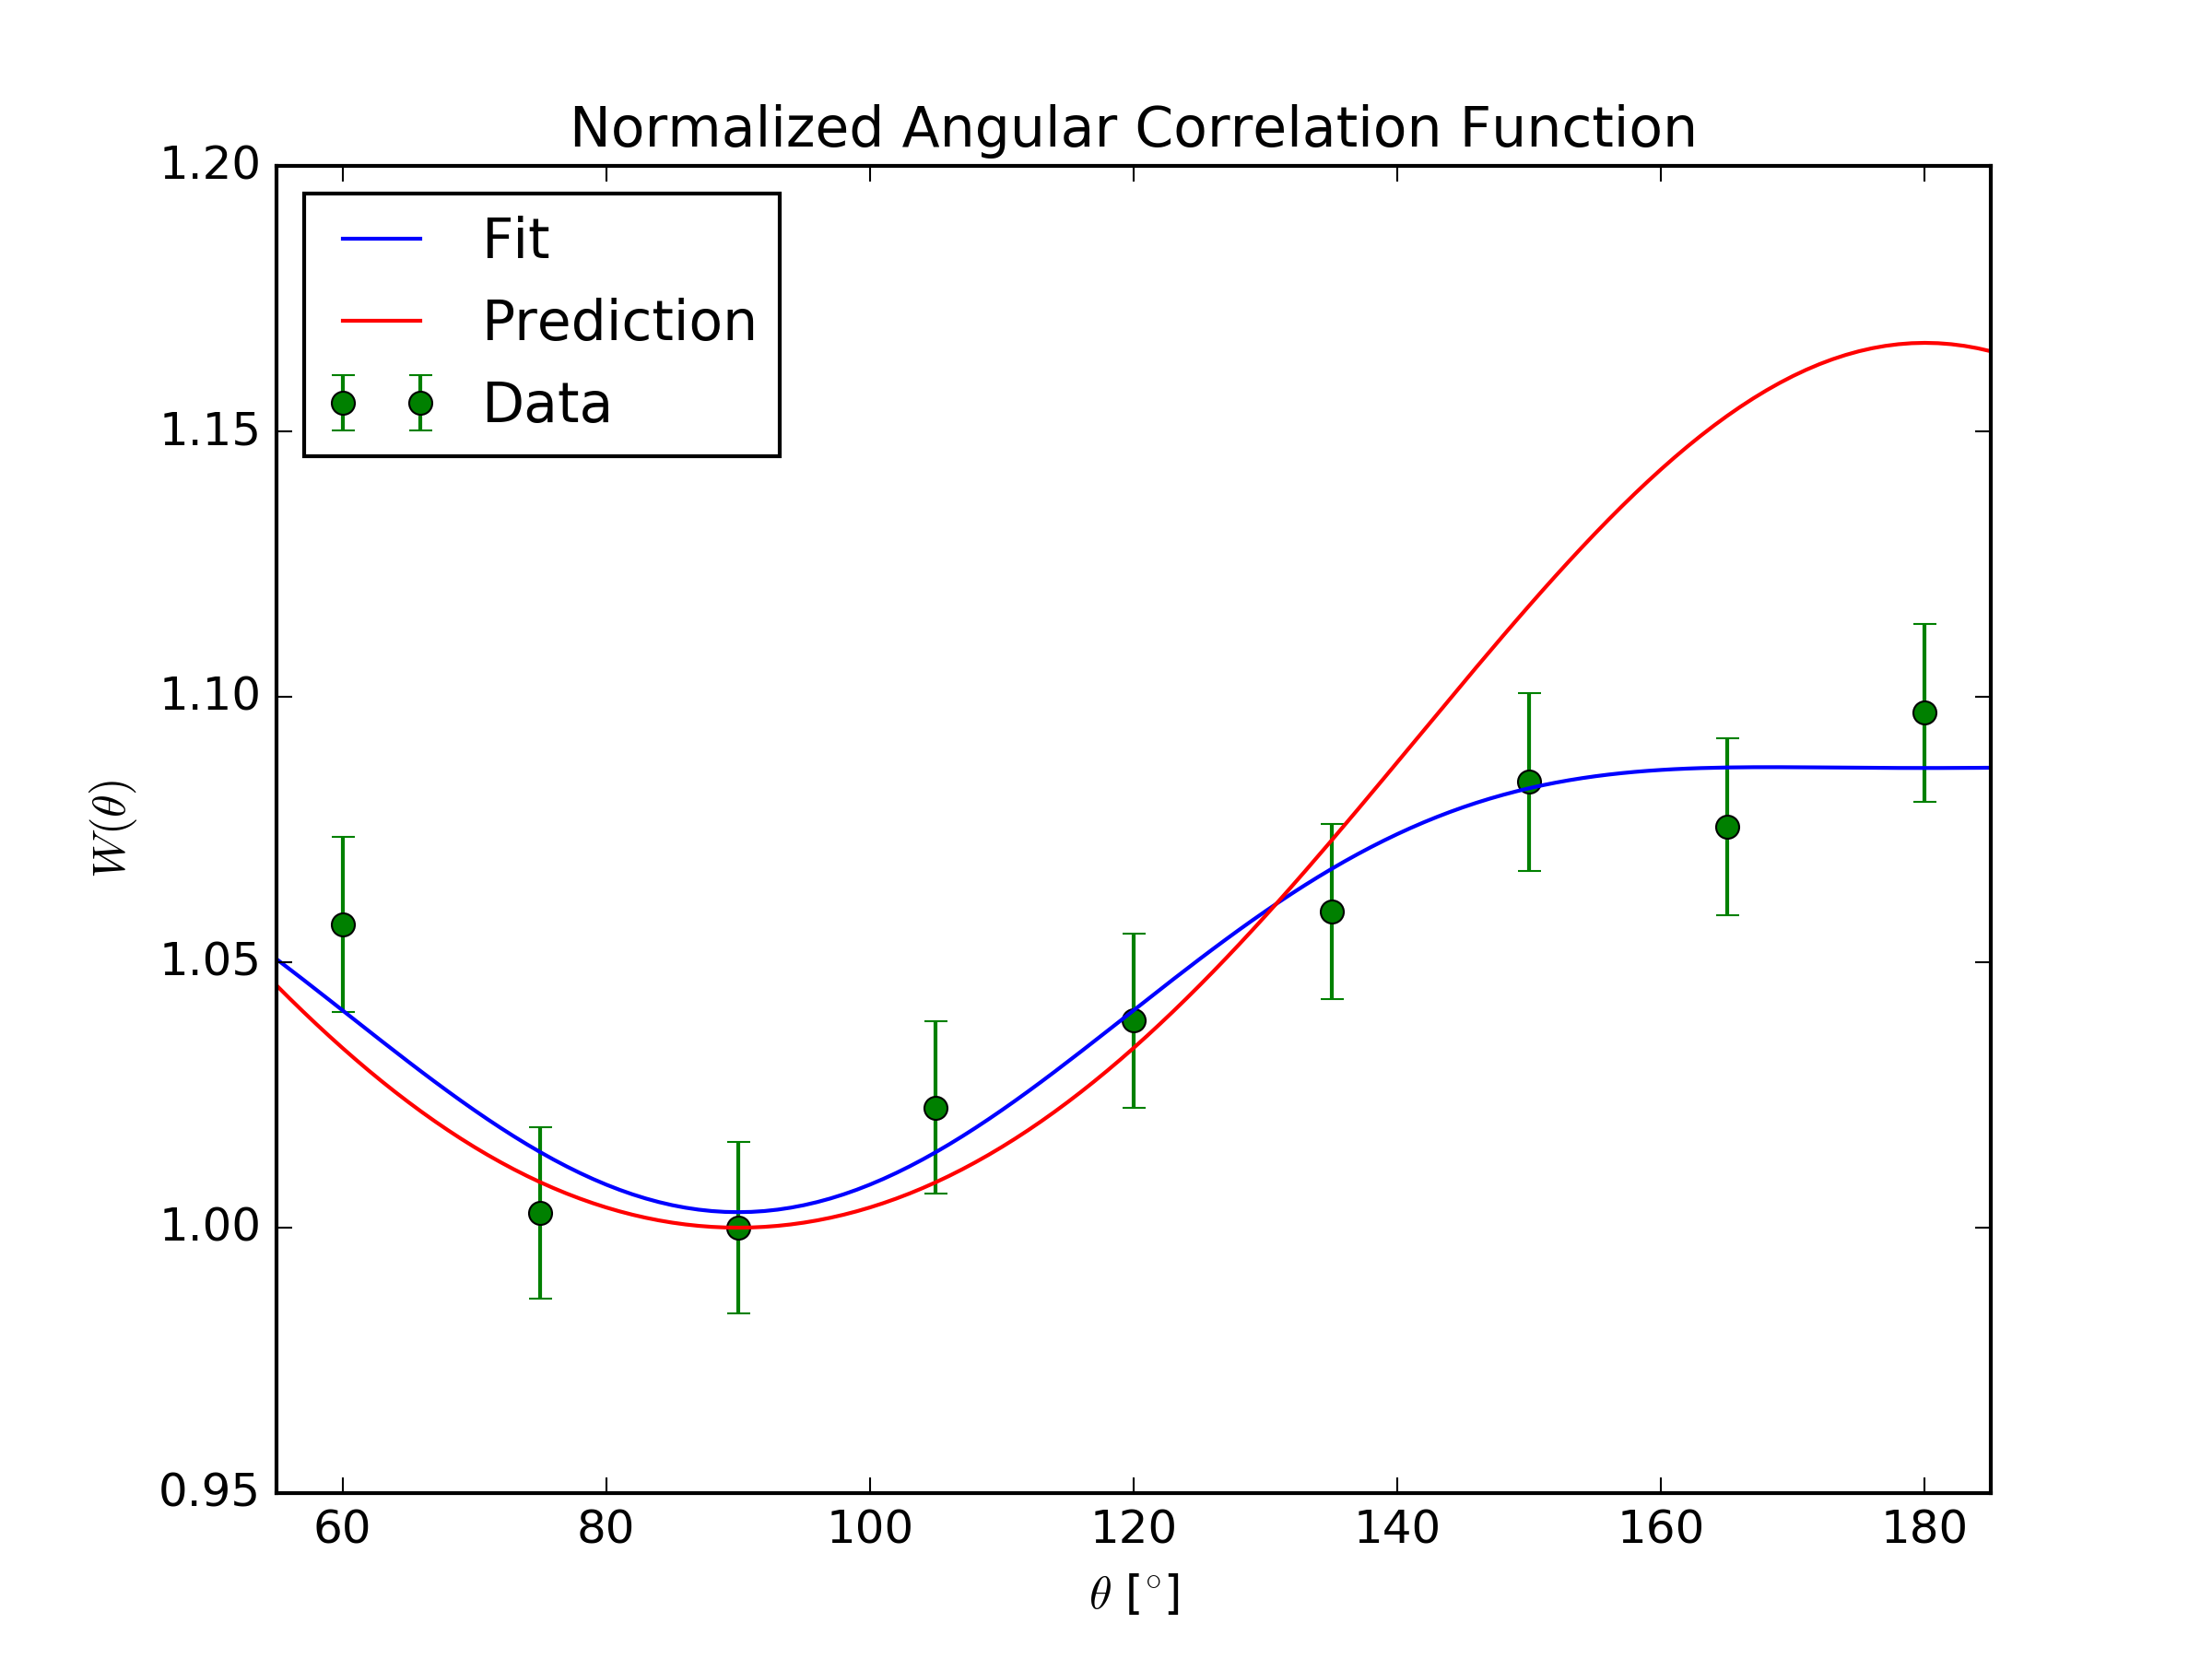
\includegraphics[scale=0.65]{plots/dist.png}
\caption[Distribution]{Normalized Angular Distribution}
\label{fig:distribution}
\end{figure}
%
For the coefficients $a_i$ we got:
%
\begin{align*}
a_0 &= 1.003 \pm 0.008\\
a_1 &= 0.157 \pm 0.049\\
a_2 &= -0.075 \pm 0.047\\
\end{align*}
%
comparing this the literature values
%
\begin{align*}
a_{0,lit} &= 1\\
a_{1,lit} &= 1/8 = 0.125\\
a_{2,lit} &= 1/24 \approx 0.042\\
\end{align*}
%
we see that $a_{0,lit}$ and $a_{1,lit}$ are within the range while $a_{2,lit}$ is not. From figure \ref{fig:distribution} it is also clearly visible that our measured data does not verify the prediction for angles starting at $\theta=135^{\circ}$. In the range of $\theta \in \left[60^{\circ},120^{\circ}\right]$ the measured data corresponds to the prediction.












\end{document}